\documentclass[10pt]{beamer}\usepackage[]{graphicx}\usepackage[]{xcolor}
% maxwidth is the original width if it is less than linewidth
% otherwise use linewidth (to make sure the graphics do not exceed the margin)
\makeatletter
\def\maxwidth{ %
  \ifdim\Gin@nat@width>\linewidth
    \linewidth
  \else
    \Gin@nat@width
  \fi
}
\makeatother

\definecolor{fgcolor}{rgb}{0.345, 0.345, 0.345}
\newcommand{\hlnum}[1]{\textcolor[rgb]{0.686,0.059,0.569}{#1}}%
\newcommand{\hlstr}[1]{\textcolor[rgb]{0.192,0.494,0.8}{#1}}%
\newcommand{\hlcom}[1]{\textcolor[rgb]{0.678,0.584,0.686}{\textit{#1}}}%
\newcommand{\hlopt}[1]{\textcolor[rgb]{0,0,0}{#1}}%
\newcommand{\hlstd}[1]{\textcolor[rgb]{0.345,0.345,0.345}{#1}}%
\newcommand{\hlkwa}[1]{\textcolor[rgb]{0.161,0.373,0.58}{\textbf{#1}}}%
\newcommand{\hlkwb}[1]{\textcolor[rgb]{0.69,0.353,0.396}{#1}}%
\newcommand{\hlkwc}[1]{\textcolor[rgb]{0.333,0.667,0.333}{#1}}%
\newcommand{\hlkwd}[1]{\textcolor[rgb]{0.737,0.353,0.396}{\textbf{#1}}}%
\let\hlipl\hlkwb

\usepackage{framed}
\makeatletter
\newenvironment{kframe}{%
 \def\at@end@of@kframe{}%
 \ifinner\ifhmode%
  \def\at@end@of@kframe{\end{minipage}}%
  \begin{minipage}{\columnwidth}%
 \fi\fi%
 \def\FrameCommand##1{\hskip\@totalleftmargin \hskip-\fboxsep
 \colorbox{shadecolor}{##1}\hskip-\fboxsep
     % There is no \\@totalrightmargin, so:
     \hskip-\linewidth \hskip-\@totalleftmargin \hskip\columnwidth}%
 \MakeFramed {\advance\hsize-\width
   \@totalleftmargin\z@ \linewidth\hsize
   \@setminipage}}%
 {\par\unskip\endMakeFramed%
 \at@end@of@kframe}
\makeatother

\definecolor{shadecolor}{rgb}{.97, .97, .97}
\definecolor{messagecolor}{rgb}{0, 0, 0}
\definecolor{warningcolor}{rgb}{1, 0, 1}
\definecolor{errorcolor}{rgb}{1, 0, 0}
\newenvironment{knitrout}{}{} % an empty environment to be redefined in TeX

\usepackage{alltt}

\usetheme[progressbar=frametitle]{metropolis}
\usecolortheme{aggie}

\usepackage{tikz}
\usepackage{graphicx}
\graphicspath{{img/}}
\usepackage{appendixnumberbeamer}

\usepackage{booktabs}
\usepackage[scale=2]{ccicons}
\usepackage[style=authoryear-comp,backend=biber]{biblatex}
%== use and define color ==%
\AtEveryCite{\color{blue}}
\addbibresource{references.bib}

\usepackage{pgfplots}
\usepackage{amsmath}
\usepackage{bm}
\usepackage{listings}
\lstset{frame=tb,
language=R,
keywordstyle=\color{blue},
alsoletter={.}
}
\usepgfplotslibrary{dateplot}

% Customize footline to include current and total slide numbers
\makeatletter

\setbeamertemplate{footline}{
  \begin{tikzpicture}[remember picture,overlay]
    % Utiliser un compteur pour sélectionner différentes images avec modulo 5
    \pgfmathtruncatemacro{\imageindex}{mod(\thepage-1,4)+1}
    \node[anchor=south west, inner sep=0pt] at (current page.south west) {
      % Insérer l'image à gauche
      \includegraphics[height=0.5cm]{img/footer/image\imageindex}
    };
    \node[anchor=south east, inner sep=0pt] at (current page.south east) {
      % Vous pouvez également ajouter d'autres éléments à droite du pied de page si nécessaire
    };
  \end{tikzpicture}
  \ifnum\c@framenumber>1%
    \hfill%
    {\fontsize{10}{12}\selectfont % Adjust the font size here
    \color{gray}%
    \insertframenumber/\inserttotalframenumber}%
  \fi%
}
\makeatother

\usepackage{xspace}
\newcommand{\themename}{\textbf{\textsc{metropolis}}\xspace}

\title{Projet: ANOVA Phylogénétique}
\subtitle{Présentation du Mercredi 10 Jan. 2024}
% \date{\today}
\date{}
\author{Alizée Geffroy, Louis Lacoste, encadrés par Mélina Gallopin et Paul Bastide}
\institute{M2 MathSV Université Paris-Saclay}
% \titlegraphic{\hfill\includegraphics[height=1.5cm]{logo.pdf}}
\IfFileExists{upquote.sty}{\usepackage{upquote}}{}
\begin{document}

\maketitle
\begin{frame}{Sommaire}
  \setbeamertemplate{section in toc}[sections numbered]
  \tableofcontents%[hideallsubsections]
\end{frame}

\section[Rappel du contexte et enjeux du projet]{Rappel du contexte et enjeux du projet}
\begin{frame}[fragile]{Contexte biologique}
\begin{itemize}
    \item Un arbre phylo avec plusieurs espèces
    \item Un trait quantitatif présent chez ces espèces
    \item Représenté par un paramètre $\mu$
\end{itemize}
Typiquement un gène dont on mesure l'expression.
Dans \textbf{\textcite{gomez-mestrePhylogeneticAnalysesReveal2012}} ces méthodes sont utilisées pour répondre à des questions d'évolution et d'ordre d'apparition de caractères chez les \emph{Anoures}.
\end{frame}
\begin{frame}{ANOVA vs ANOVA phylogénétique}
  \begin{equation*}
    \bm{Y} = \bm{X}\beta+ \bm{\sigma} \bm{E}  \text{  où  } \bm{X}=(1,1_2, ..., 1_K) \text{   et   }\beta = (\mu _1, \beta _2, ..., \beta _K)^T
  \end{equation*}
    \begin{columns}

       \column{0.5\textwidth}
       \begin{center}
       Anova
       \end{center}
    \begin{equation*}
    \bm{E} \sim \mathcal{N}(0_n, \bm{Id})
      \end{equation*} 
      
    \column{0.5\textwidth}
    \begin{center}
       Anova phylogénétique 
       \end{center}
    \begin{equation*}
    \bm{E} \sim \mathcal{N}(0_n, \bm{V})
    \end{equation*}
  \end{columns}
    \begin{center}
        Estimateur du max. de vraisemblance
    \end{center}
  \begin{columns}
      \column{0.5\textwidth}
      \centering
        $\hat{\beta} = (\bm{X}^{T}\bm{X})^{-1}\bm{X}^{T}\bm{Y}$\\
        $\hat{\sigma}^2 =  \frac{1}{n-p} (\bm{Y} - \bm{X}\hat{\beta})^T(\bm{Y} - \bm{X}\hat{\beta})$
        % Finir
      \column{0.5\textwidth}
      \centering
        $\hat{\beta}_{phylo} = (\bm{X}^{T}\bm{V}^{-1}\bm{X})^{-1}\bm{X}^{T}\bm{V}^{-1}\bm{Y}$\\
        $\hat{\sigma}_{phylo}^2 =  \frac{1}{n-p} (\bm{Y} - \bm{X}\hat{\beta})^T\bm{V}^{-1}(\bm{Y} - \bm{X}\hat{\beta})$
  \end{columns}
  

    \footnotetext{Pour l'ANOVA Phylogénétique, nos références sont \cite{bastideContinuousTraitEvolution} et \cite{bastideModelesEvolutionCaracteres2022} et pour l'ANOVA, \cite{belModeleLineaireSes}.}
Objectif : Comparer les méthodes Anova et Anova phylogénétique
\end{frame}
\begin{frame}{Différents types de groupes}
\begin{columns}
    \begin{column}{0.5\textwidth}
        \begin{figure}
        \centering
    On forme des groupes \textbf{en lien avec la phylogénie}.
        \includegraphics[scale=0.32]{img/group_phylo_tree.png}
        \caption{Arbre phylogénétique et groupes concordants}
        \label{fig:phylo_matching}
    \end{figure}
    \end{column}
    \begin{column}{0.5\textwidth}
        \begin{figure}
            \centering
    On forme des groupes qui ne sont \textbf{pas phylogénétiques}.
            \includegraphics[scale=0.32]{img/group_nonphylo_tree.png}
            \caption{Arbre phylogénétique et groupes non concordants}
            \label{fig:phylo-non-matching}
        \end{figure}
    \end{column}
\end{columns}

\end{frame}

% \begin{frame}[fragile]{Cas 1}
% Anova classique VS Anova phylogénétique
% \newline
% Voir les impacts de leur utilisation dans 2 cas:
% \begin{itemize}
%     \item 1) On attribue des groupes au hasard -> les groupes ne sont pas liés à l'info phylogénétique
%     \item  2) Les groupes sont définis en lien avec la phylogénie (des espèces proches ont un trait identique ou proche) -> la phylogénie donne une information sur les groupes
% \end{itemize}
% #METTRE LES IMAGES

% Objectifs : Comparer les méthodes Anova et Anova phylogénétique
% \end{frame}
% \begin{frame}[fragile]{Nos hypothèses}
% \newline
% \begin{itemize}
%     \item 1) Groupes non liés à l'info phylogénétique -> l'Anova phylogénétique sera égale voir moins bonne que l'Anova classique
%     \item 2) Phylogénie donne une information sur les groupes -> l'Anova phylogénétique va donner de meilleurs résultats que la classique en prenant en compte la structure de l'arbre
% \end{itemize}
% \end{frame}

\begin{frame}[fragile]{Les résultats, 1}
\begin{figure}
    \centering
    \includegraphics[scale=0.32]{img/simulation_power_pure_BM.png}
    \caption{Avec de la variabilité purement phylogénétique}
    \label{fig:only_phylo_error}
\end{figure}
\end{frame}

\begin{frame}[fragile]{Les résultats, 2}
\begin{figure}
    \centering
    \includegraphics[scale=0.32]{img/simulation_power_pure_both_error.png}
    \caption{Avec de la variabilité phylogénétique et d'erreur de mesure}
    \label{fig:with_phylo_and_measure_error}
\end{figure}
\end{frame}

\begin{frame}[fragile]{Ce qu'il se passe vraiment}
L'observation se présente sous la forme suivante si réécrite en tant que modèle à effets mixtes :
$$\bm{Y} = \bm{X}\beta + \underbrace{\bm{E}}_{\bm{Z} u + \epsilon} $$
avec $\bm{Z} u \sim \mathcal{N}(0,\sigma^2_{phylo}V)$, $\epsilon \sim \mathcal{N}(0,\sigma^2_{mesure}\bm{Id})$ et $Var(\bm{E})=\sigma^2_{phylo} (V + \lambda\bm{Id})$ où $\lambda=\frac{\sigma^2_{mesure}}{\sigma^2_{phylo}}$

Les méthodes d'ANOVA phylogénétique telles qu'implémentées dans \texttt{phylolm} estiment les paramètres $\sigma^2_{mesure}$ d'erreur de mesure et $\sigma^2_{phylo}$ de variabilité dûe à la phylogénie.\\
\emph{Mais} une fois estimé, lors du test de Fisher les paramètres sont considérés comme si non estimés.


Le but ici est donc d'utiliser l'approximation de \textcite{satterthwaiteApproximateDistributionEstimates1946} afin de calculer les degrés de libertés du test de loi de Fisher à réaliser.
\end{frame}

\section{Conclusions et perspectives}
\begin{frame}{Avec des données individuelles}
\begin{center}
\usetikzlibrary{trees}
\scalebox{0.75}{
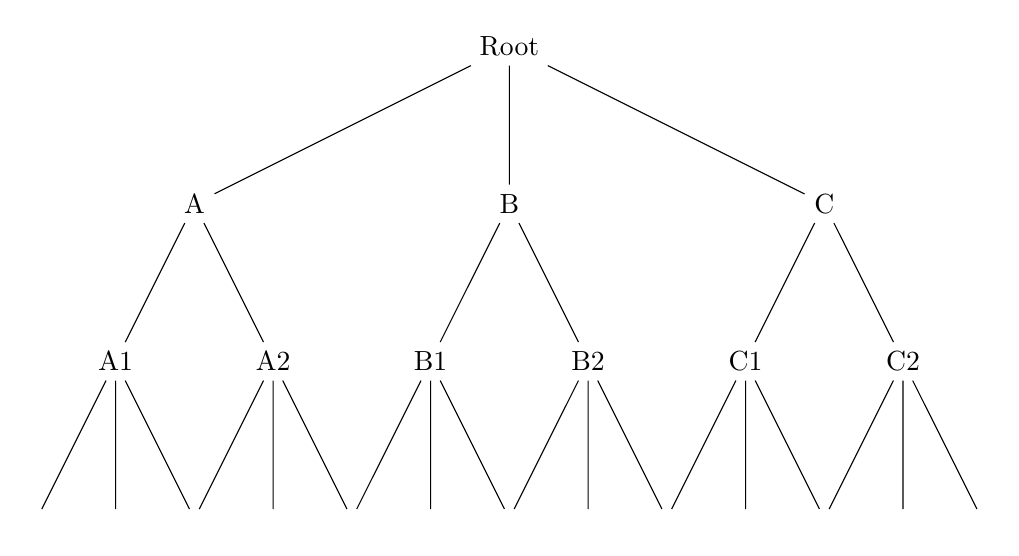
\begin{tikzpicture}[level distance=2cm,
                    level 1/.style={sibling distance=4cm},
                    level 2/.style={sibling distance=2cm},
                    level 3/.style={sibling distance=1cm}]
  \node {Root}
    child {
    node {A}
      child {node {A1}
        child {node {}}
        child {node {}}
        child {node {}}
      }
      child {node {A2}
        child {node {}}
        child {node {}}
        child {node {}}
      }
    }
    child {
    node {B}
      child {node {B1}
        child {node {}}
        child {node {}}
        child {node {}}
      }
      child {node {B2}
        child {node {}}
        child {node {}}
        child {node {}}
      }
    }    
    child {
    node {C}
      child {node {C1}
        child {node {}}
        child {node {}}
        child {node {}}
      }
      child {node {C2}
        child {node {}}
        child {node {}}
        child {node {}}
      }
    };
\end{tikzpicture}
}\\
\end{center}
Le package \texttt{phylolimma}\footnote{Disponible sur \url{https://github.com/pbastide/phylolimma/}} permet de compléter un arbre existant en ajoutant les sous-branches au bout.\\
Nous voulons obtenir une méthode d'estimation des paramètres et l'implémenter sur ce type d'arbre.
\end{frame}
\begin{frame}{Perspectives}
    \begin{itemize}
        \item Implémenter le test statistique correspondant à l'approximation de Satterthwaite.
        \item Implémenter le test de ratio de log-vraisemblance.
        \item Implémenter avec plusieurs individus par espèces
    \end{itemize}
    \begin{block}{Objectif principal}
    Trouver un test robuste et rapide, applicable à des milliers de données d'expressions de gènes mesurées dans une expérience RNAseq typique.
    \end{block}

\end{frame}

\section{Références et appendices}
\begin{frame}[allowframebreaks]{References}

    \printbibliography
  % \bibliographystyle{abbrv}

\end{frame}

\appendix

\begin{frame}[allowframebreaks]{Code pour les simulations}
 Le code pour les simulations est disponible sur notre dépôt GitHub : \\
\begin{center}
    \url{https://github.com/Polarolouis/anova-phylogenetique-projet-msv/}
\end{center}
\end{frame}

% \begin{frame}[fragile]{Metropolis}

%   The \themename theme is a Beamer theme with minimal visual noise
%   inspired by the \href{https://github.com/hsrmbeamertheme/hsrmbeamertheme}{\textsc{hsrm} Beamer
%   Theme} by Benjamin Weiss.

%   Enable the theme by loading

%   \begin{verbatim}    \documentclass{beamer}
%     \usetheme{metropolis}\end{verbatim}

%   Note, that you have to have Mozilla's \emph{Fira Sans} font and XeTeX
%   installed to enjoy this wonderful typography.
% \end{frame}
% \begin{frame}[fragile]{Sections}
%   Sections group slides of the same topic

%   \begin{verbatim}    \section{Elements}\end{verbatim}

%   for which \themename provides a nice progress indicator \ldots
  
% \end{frame}

% \section{Titleformats}

% \begin{frame}{Metropolis titleformats}
% 	\themename supports 4 different titleformats:
% 	\begin{itemize}
% 		\item Regular
% 		\item \textsc{Smallcaps}
% 		\item \textsc{allsmallcaps}
% 		\item ALLCAPS
% 	\end{itemize}
% 	They can either be set at once for every title type or individually.
% \end{frame}

% \subsection{Tricks}

% {
%     \metroset{titleformat frame=smallcaps}
% \begin{frame}{Small caps}
% 	This frame uses the \texttt{smallcaps} titleformat.

% 	\begin{alertblock}{Potential Problems}
% 		Be aware, that not every font supports small caps. If for example you typeset your presentation with pdfTeX and the Computer Modern Sans Serif font, every text in smallcaps will be typeset with the Computer Modern Serif font instead.
% 	\end{alertblock}
% \end{frame}
% }

% {
% \metroset{titleformat frame=allsmallcaps}
% \begin{frame}{All small caps}
% 	This frame uses the \texttt{allsmallcaps} titleformat.

% 	\begin{alertblock}{Potential problems}
% 		As this titleformat also uses smallcaps you face the same problems as with the \texttt{smallcaps} titleformat. Additionally this format can cause some other problems. Please refer to the documentation if you consider using it.

% 		As a rule of thumb: Just use it for plaintext-only titles.
% 	\end{alertblock}
% \end{frame}
% }

% {
% \metroset{titleformat frame=allcaps}
% \begin{frame}{All caps}
% 	This frame uses the \texttt{allcaps} titleformat.

% 	\begin{alertblock}{Potential Problems}
% 		This titleformat is not as problematic as the \texttt{allsmallcaps} format, but basically suffers from the same deficiencies. So please have a look at the documentation if you want to use it.
% 	\end{alertblock}
% \end{frame}
% }

% \section{Elements}

% \begin{frame}[fragile]{Typography}
%       \begin{verbatim}The theme provides sensible defaults to
% \emph{emphasize} text, \alert{accent} parts
% or show \textbf{bold} results.\end{verbatim}

%   \begin{center}becomes\end{center}

%   The theme provides sensible defaults to \emph{emphasize} text,
%   \alert{accent} parts or show \textbf{bold} results.
% \end{frame}

% \begin{frame}{Font feature test}
%   \begin{itemize}
%     \item Regular
%     \item \textit{Italic}
%     \item \textsc{SmallCaps}
%     \item \textbf{Bold}
%     \item \textbf{\textit{Bold Italic}}
%     \item \textbf{\textsc{Bold SmallCaps}}
%     \item \texttt{Monospace}
%     \item \texttt{\textit{Monospace Italic}}
%     \item \texttt{\textbf{Monospace Bold}}
%     \item \texttt{\textbf{\textit{Monospace Bold Italic}}}
%   \end{itemize}
% \end{frame}

% \begin{frame}{Lists}
%   \begin{columns}[T,onlytextwidth]
%     \column{0.33\textwidth}
%       Items
%       \begin{itemize}
%         \item Milk \item Eggs \item Potatos
%       \end{itemize}

%     \column{0.33\textwidth}
%       Enumerations
%       \begin{enumerate}
%         \item First, \item Second and \item Last.
%       \end{enumerate}

%     \column{0.33\textwidth}
%       Descriptions
%       \begin{description}
%         \item[PowerPoint] Meeh. \item[Beamer] Yeeeha.
%       \end{description}
%   \end{columns}
% \end{frame}
% \begin{frame}{Animation}
%   \begin{itemize}[<+- | alert@+>]
%     \item \alert<4>{This is\only<4>{ really} important}
%     \item Now this
%     \item And now this
%   \end{itemize}
% \end{frame}
% \begin{frame}{Figures}
%   \begin{figure}
%     \newcounter{density}
%     \setcounter{density}{20}
%     \begin{tikzpicture}
%       \def\couleur{alerted text.fg}
%       \path[coordinate] (0,0)  coordinate(A)
%                   ++( 90:5cm) coordinate(B)
%                   ++(0:5cm) coordinate(C)
%                   ++(-90:5cm) coordinate(D);
%       \draw[fill=\couleur!\thedensity] (A) -- (B) -- (C) --(D) -- cycle;
%       \foreach \x in {1,...,40}{%
%           \pgfmathsetcounter{density}{\thedensity+20}
%           \setcounter{density}{\thedensity}
%           \path[coordinate] coordinate(X) at (A){};
%           \path[coordinate] (A) -- (B) coordinate[pos=.10](A)
%                               -- (C) coordinate[pos=.10](B)
%                               -- (D) coordinate[pos=.10](C)
%                               -- (X) coordinate[pos=.10](D);
%           \draw[fill=\couleur!\thedensity] (A)--(B)--(C)-- (D) -- cycle;
%       }
%     \end{tikzpicture}
%     \caption{Rotated square from
%     \href{http://www.texample.net/tikz/examples/rotated-polygons/}{texample.net}.}
%   \end{figure}
% \end{frame}
% \begin{frame}{Tables}
%   \begin{table}
%     \caption{Largest cities in the world (source: Wikipedia)}
%     \begin{tabular}{lr}
%       \toprule
%       City & Population\\
%       \midrule
%       Mexico City & 20,116,842\\
%       Shanghai & 19,210,000\\
%       Peking & 15,796,450\\
%       Istanbul & 14,160,467\\
%       \bottomrule
%     \end{tabular}
%   \end{table}
% \end{frame}
% \begin{frame}{Blocks}
%   Three different block environments are pre-defined and may be styled with an
%   optional background color.

%   \begin{columns}[T,onlytextwidth]
%     \column{0.5\textwidth}
%       \begin{block}{Default}
%         Block content.
%       \end{block}

%       \begin{alertblock}{Alert}
%         Block content.
%       \end{alertblock}

%       \begin{exampleblock}{Example}
%         Block content.
%       \end{exampleblock}

%     \column{0.5\textwidth}

%       \metroset{block=fill}

%       \begin{block}{Default}
%         Block content.
%       \end{block}

%       \begin{alertblock}{Alert}
%         Block content.
%       \end{alertblock}

%       \begin{exampleblock}{Example}
%         Block content.
%       \end{exampleblock}

%   \end{columns}
% \end{frame}
% \begin{frame}{Math}
%   \begin{equation*}
%     e = \lim_{n\to \infty} \left(1 + \frac{1}{n}\right)^n
%   \end{equation*}
% \end{frame}
% \begin{frame}{Line plots}
%   \begin{figure}
%     \begin{tikzpicture}
%       \begin{axis}[
%         mlineplot,
%         width=0.9\textwidth,
%         height=6cm,
%       ]

%         \addplot {sin(deg(x))};
%         \addplot+[samples=100] {sin(deg(2*x))};

%       \end{axis}
%     \end{tikzpicture}
%   \end{figure}
% \end{frame}
% \begin{frame}{Bar charts}
%   \begin{figure}
%     \begin{tikzpicture}
%       \begin{axis}[
%         mbarplot,
%         xlabel={Foo},
%         ylabel={Bar},
%         width=0.9\textwidth,
%         height=6cm,
%       ]

%       \addplot plot coordinates {(1, 20) (2, 25) (3, 22.4) (4, 12.4)};
%       \addplot plot coordinates {(1, 18) (2, 24) (3, 23.5) (4, 13.2)};
%       \addplot plot coordinates {(1, 10) (2, 19) (3, 25) (4, 15.2)};

%       \legend{lorem, ipsum, dolor}

%       \end{axis}
%     \end{tikzpicture}
%   \end{figure}
% \end{frame}
% \begin{frame}{Quotes}
%   \begin{quote}
%     Veni, Vidi, Vici
%   \end{quote}
% \end{frame}

% {%
% \setbeamertemplate{frame footer}{My custom footer}
% \begin{frame}[fragile]{Frame footer}
%     \themename defines a custom beamer template to add a text to the footer. It can be set via
%     \begin{verbatim}\setbeamertemplate{frame footer}{My custom footer}\end{verbatim}
% \end{frame}
% }

% \begin{frame}{References}
%   Some references to showcase [allowframebreaks] \cite{knuth92,ConcreteMath,Simpson,Er01,greenwade93}
% \end{frame}

% \section{Conclusion}

% \begin{frame}{Summary}

%   Get the source of this theme and the demo presentation from

%   \begin{center}\url{github.com/matze/mtheme}\end{center}

%   The theme \emph{itself} is licensed under a
%   \href{http://creativecommons.org/licenses/by-sa/4.0/}{Creative Commons
%   Attribution-ShareAlike 4.0 International License}.

%   \begin{center}\ccbysa\end{center}

% \end{frame}

% {\setbeamercolor{palette primary}{fg=ag-blue, bg=ag-beige}
% \begin{frame}[standout]
%   Questions?
% \end{frame}
% }

% \appendix

% \begin{frame}[fragile]{Backup slides}
%   Sometimes, it is useful to add slides at the end of your presentation to
%   refer to during audience questions.

%   The best way to do this is to include the \verb|appendixnumberbeamer|
%   package in your preamble and call \verb|\appendix| before your backup slides.

%   \themename will automatically turn off slide numbering and progress bars for
%   slides in the appendix.
% \end{frame}


\end{document}
